\section{Systematic Impacts}
\label{sec:Impacts}

The systematic impacts for the Run 2 combination of the Semi-Leptonic, Fully-Hadronic and Fully-Leptonic categories combined
with Single Higgs processes modeled in all categories are shown in Figures \ref{fig:Impacts_Run2_expected-1} , \ref{fig:Impacts_Run2_expected-2} , \ref{fig:Impacts_Run2_expected-3} , \ref{fig:Impacts_Run2_expected-4} , where signal strength is set to the expected limit.    

\textbf{Note:} unconstrained systematics have been
removed from these impact plots in order to be able to view the impacts of other systematics. 

In addition, the largest impact in all cases due to the HH theory uncertainty, 
including the ggHH QCD scale uncertainty and top mass uncertainty amounting to a log normal uncertainty of +6\% / -23\%, has been removed so that the other impacts are more visible. 

\begin{figure}[h!]
    \centering
    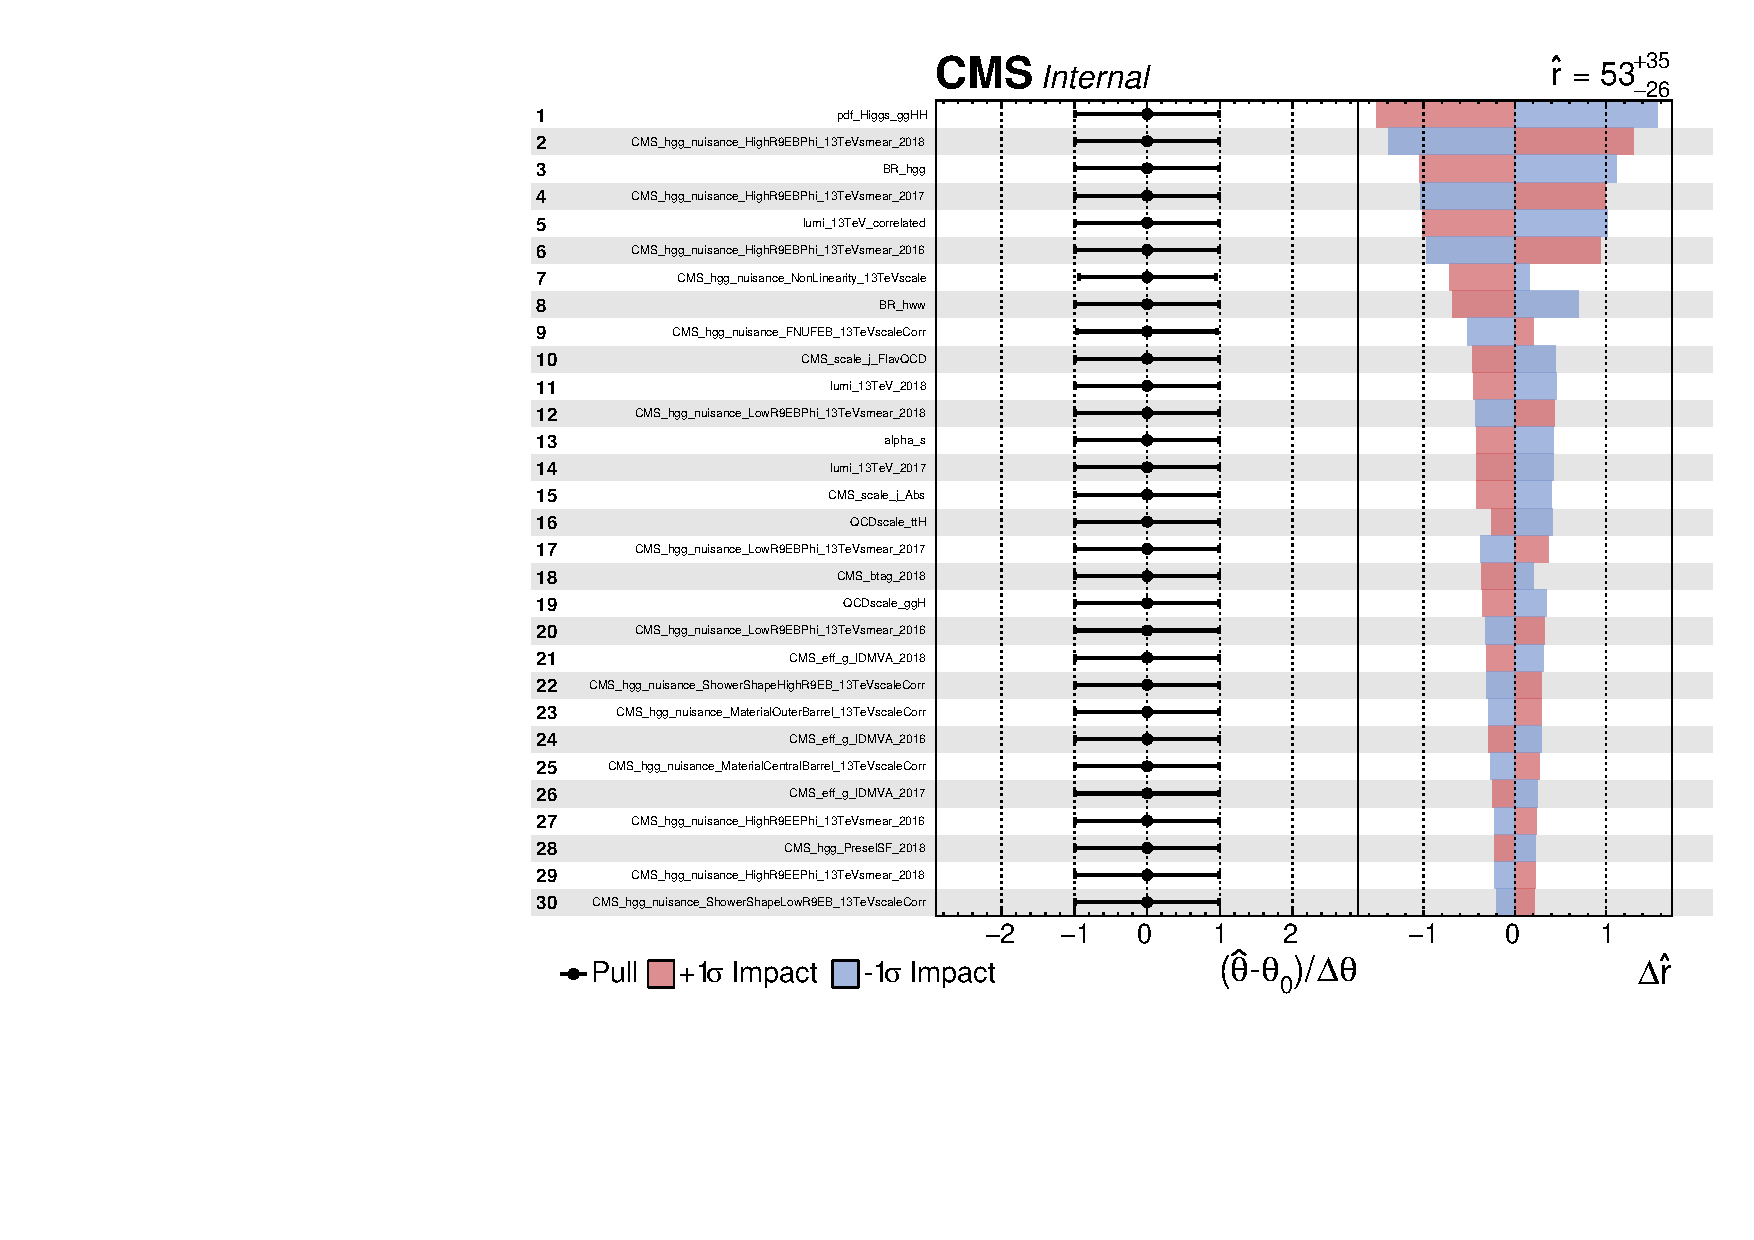
\includegraphics[page=1, width=\textwidth]{Sections/HHWWgg/images/Impacts/HHWWgg_Impacts_expected.pdf}
    \caption{Combined Run2 Expected Systematic Impacts: Page 1}
    \label{fig:Impacts_Run2_expected-1}
\end{figure}

\newpage
\begin{figure}[h!]
    \centering
    \includegraphics[page=2, width=\textwidth]{Sections/HHWWgg/images/Impacts/HHWWgg_Impacts_expected.pdf}
    \caption{Combined Run2 Expected Systematic Impacts: Page 2}
    \label{fig:Impacts_Run2_expected-2}
\end{figure}

\newpage
\begin{figure}[h!]
    \centering
    \includegraphics[page=3, width=\textwidth]{Sections/HHWWgg/images/Impacts/HHWWgg_Impacts_expected.pdf}
    \caption{Combined Run2 Expected Systematic Impacts: Page 3}
    \label{fig:Impacts_Run2_expected-3}
\end{figure}

\newpage
\begin{figure}[h!]
    \centering
    \includegraphics[page=4, width=\textwidth]{Sections/HHWWgg/images/Impacts/HHWWgg_Impacts_expected.pdf}
    \caption{Combined Run2 Expected Systematic Impacts: Page 4}
    \label{fig:Impacts_Run2_expected-4}
\end{figure}


